\documentclass[10pt]{article}
\usepackage[margin=0.85in]{geometry}
\usepackage{graphicx}
\usepackage{booktabs}
\usepackage{hyperref}
\usepackage{amsmath}
\usepackage{caption}
\usepackage{titlesec}
\usepackage{fontspec}
\newfontfamily\devanagarifont{Noto Sans Devanagari}

\titlespacing*{\section}{0pt}{6pt}{3pt}
\titlespacing*{\subsection}{0pt}{4pt}{2pt}
\setlength{\textfloatsep}{4pt plus 1pt minus 1pt}
\setlength{\intextsep}{4pt plus 1pt minus 1pt}
\setlength{\abovecaptionskip}{2pt}
\setlength{\belowcaptionskip}{2pt}
\setlength{\parskip}{1pt}
\setlength{\tabcolsep}{4pt}
\renewcommand{\arraystretch}{0.92}

\title{\vspace{-1.5em}Building and Analyzing Monolingual Transformer Language Models in Hindi and Nepali}
\author{Md Taufique Hussain}
\date{}

\begin{document}
\maketitle
\vspace{-2em}

\section*{Introduction}

For this project I built two language models from scratch, one for Hindi and one for Nepali. Hindi is the higher-resource language (Model H) and Nepali is the lower-resource one (Model L), picked from the list the assignment allows. Everything is separate for the two languages: the data, the tokenizer, the model weights. I did the data collection, cleaning, tokenizer training, the Transformer code itself, pretraining, the reasoning finetune, and every evaluation, for both languages, on my own.

This report puts the results from all three phases in one place and tries to explain why Hindi keeps coming out a bit ahead of Nepali, stage after stage, and what that gap is actually made of.

\section{Phase 1: Data Collection and Tokenizer}

\subsection{Where the data came from}

For each language I mixed text I crawled myself with a public corpus, IndicCorpV2. For Hindi that meant four news sites (zeenews.india.com, indiatv.in, jagran.com, patrika.com) plus Hindi Wikipedia through the MediaWiki API, on top of the Hindi part of IndicCorpV2. Nepali got the same treatment: four news sites (khabarhub.com, dcnepal.com, karobardaily.com, nepalnews.com), Nepali Wikipedia, and the Nepali part of IndicCorpV2. I tried a fifth Nepali site, nepalpress.com, but my crawler kept coming back with zero URLs even though the sitemap looked fine when I opened it in a browser. Turned out to be a Cloudflare rule. I didn't bother building a workaround for one site out of five.

Both corpora go through the same cleaning steps: Unicode normalization, drop anything under 200 characters, a script check (at least 70\% Devanagari, at most 15\% Latin), a filter for repeated boilerplate text, a profanity filter, then exact and near-duplicate removal. Near-duplicate removal only runs on the crawled part, not on IndicCorp. IndicCorp already comes deduplicated, and running my own dedup on several million more documents would have needed more RAM than I had.

\begin{table}[h]
\centering
\small
\begin{tabular}{lrr}
\toprule
 & Hindi (Model H) & Nepali (Model L) \\
\midrule
Raw documents collected & 8,878,491 & 12,159,484 \\
Documents kept after cleaning & 4,686,338 (52.8\%) & 5,154,832 (42.4\%) \\
Train / val / test documents & 4,592,126 / 47,287 / 46,925 & 5,051,679 / 51,458 / 51,695 \\
\bottomrule
\end{tabular}
\caption{Corpus sizes after cleaning, both languages.}
\end{table}

Nepali started with more raw documents but kept less of them. Almost all of that comes from the 200-character filter. More of Nepali's raw IndicCorp text turned out to be short fragments, not full articles. I don't think that's a bug in my code, just a real difference in how the two IndicCorpV2 shards were put together.

\begin{figure}[h]
\centering
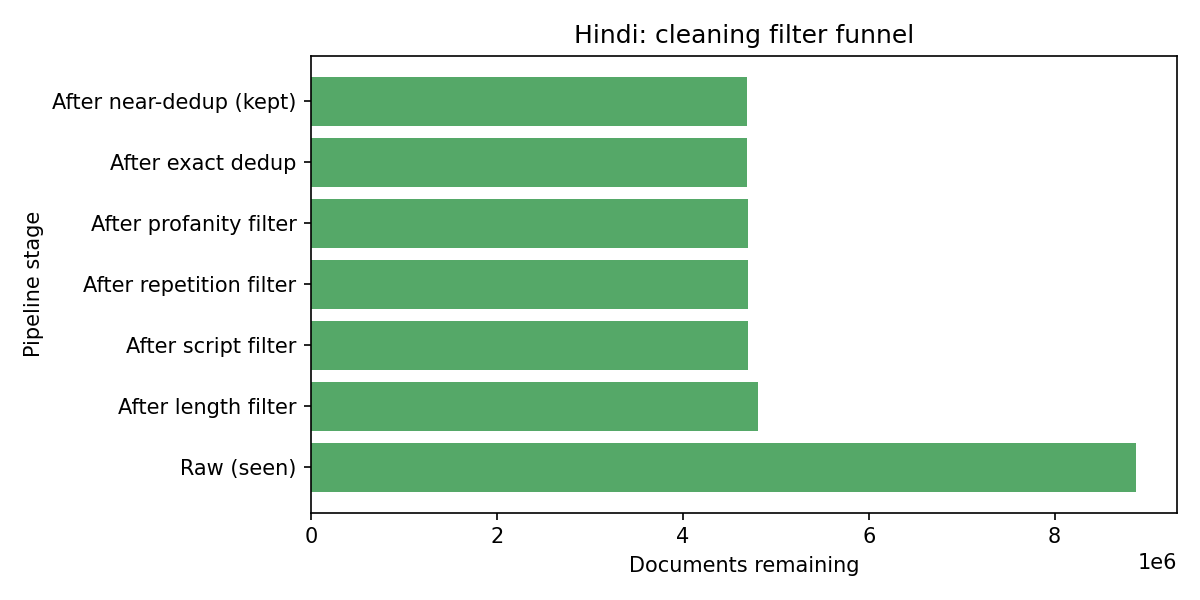
\includegraphics[width=0.32\textwidth]{../phase1/plots/filter_funnel_hindi.png}
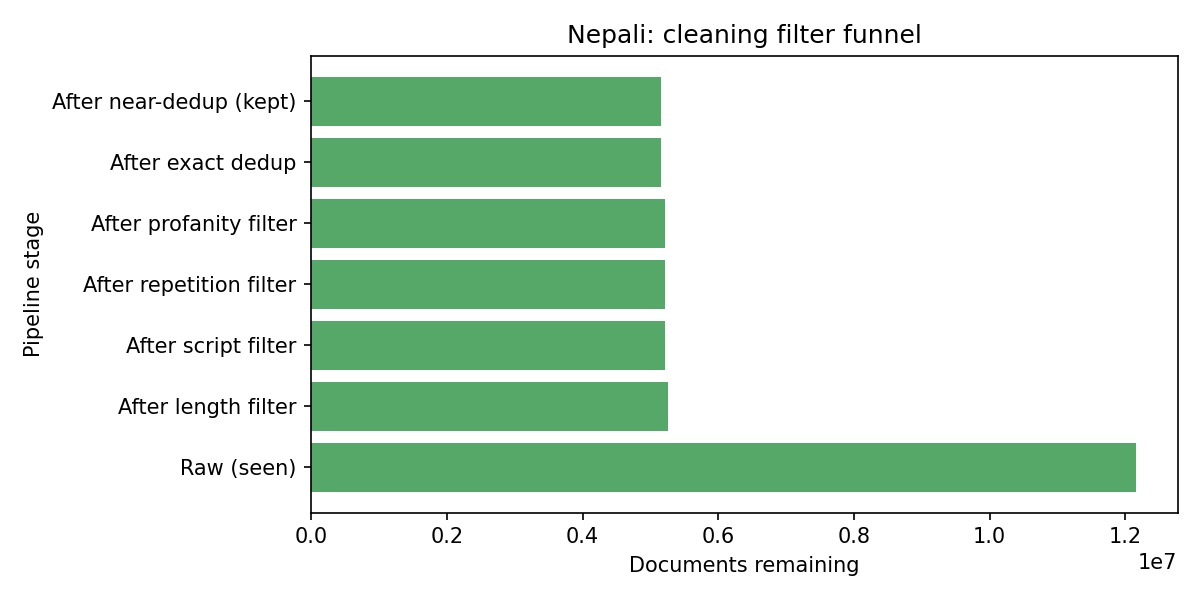
\includegraphics[width=0.32\textwidth]{../phase1/plots/filter_funnel_nepali.png}
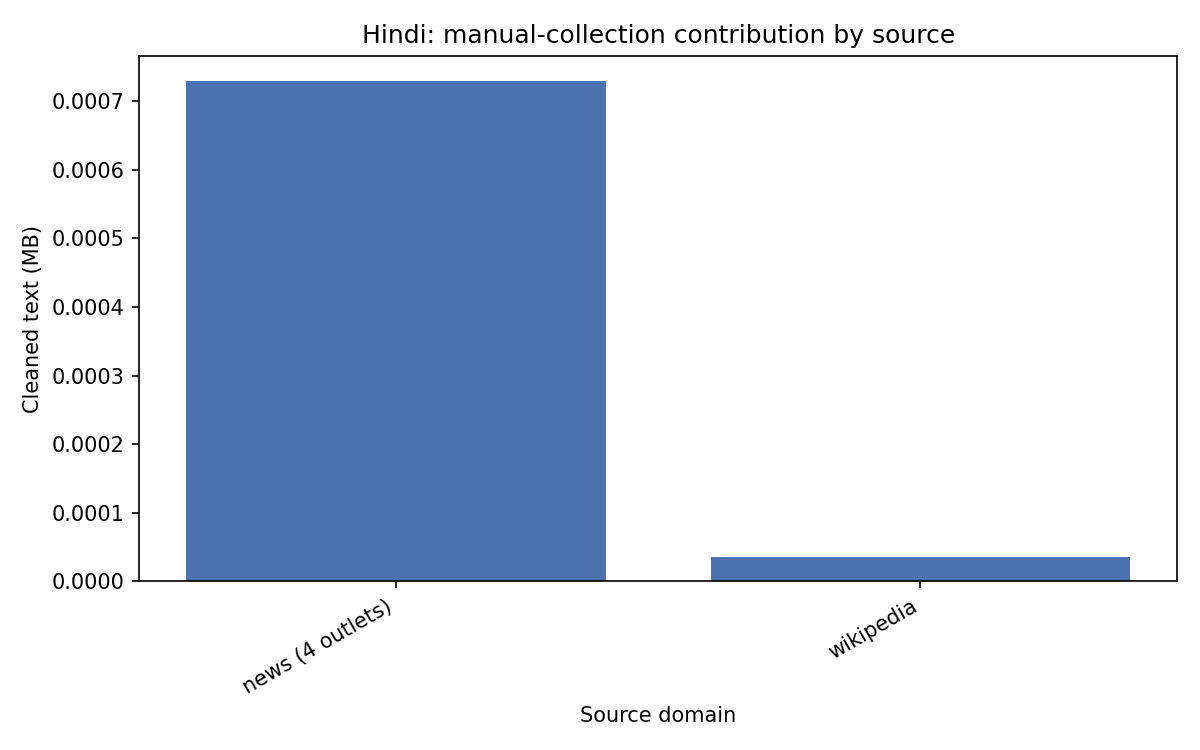
\includegraphics[width=0.32\textwidth]{../phase1/plots/source_contribution_hindi.png}
\caption{Cleaning funnel (Hindi, Nepali) and Hindi's manual-source contribution.}
\end{figure}

Splits come from hashing each document's ID (\texttt{sha256(doc\_id) \% 100}), so re-running the pipeline always gives the same split, and a document can never land in two splits at once.

\subsection{Tokenizer}

I trained a separate SentencePiece Unigram tokenizer per language, with byte-fallback on so nothing is ever truly unrepresentable. I went with Unigram instead of BPE because both languages inflect a lot (case endings, verb forms), and Unigram tends to land on subword pieces closer to actual meaningful chunks than BPE's merge rule does.

To pick a vocabulary size I swept a few values and measured fertility (average characters per token) on held-out text:

\begin{table}[h]
\centering
\small
\begin{tabular}{rrr}
\toprule
Vocabulary size & Hindi fertility & Nepali fertility \\
\midrule
5,000 & 3.53 & 3.77 \\
7,000 & 3.73 & 4.04 \\
9,000 & 3.86 & 4.22 \\
16,000 & 4.11 & 4.57 \\
24,000 & 4.23 & 4.76 \\
32,000 & 4.30 & 4.88 \\
\bottomrule
\end{tabular}
\caption{Fertility (characters per token) at different vocabulary sizes.}
\end{table}

\begin{figure}[h]
\centering
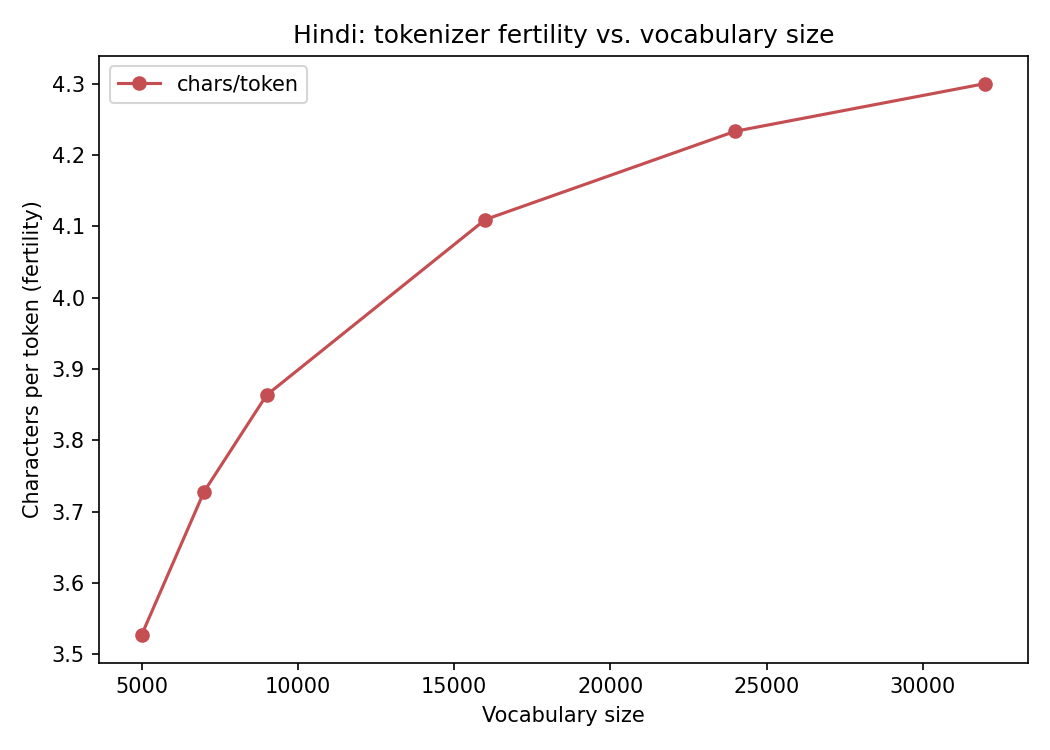
\includegraphics[width=0.4\textwidth]{../phase1/plots/fertility_sweep_hindi.png}
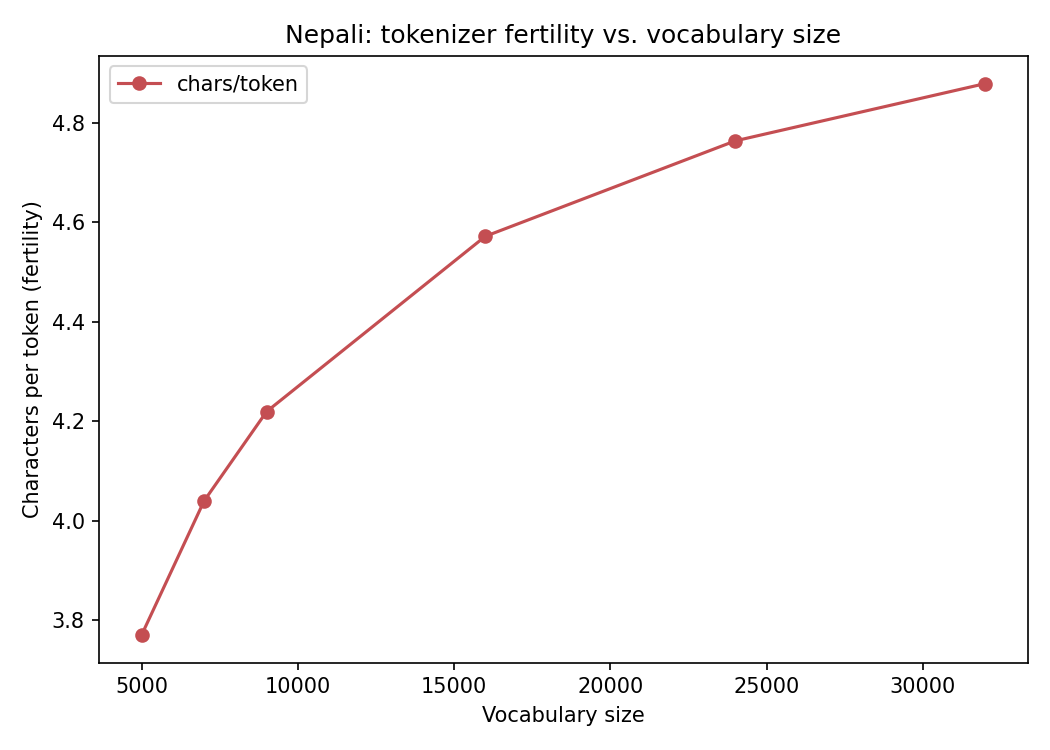
\includegraphics[width=0.4\textwidth]{../phase1/plots/fertility_sweep_nepali.png}
\caption{Fertility vs. vocabulary size sweep, Hindi (left) and Nepali (right).}
\end{figure}

I went with 9,000 for both. Moving from 5,000 to 9,000 only adds about 0.8M parameters out of a 25M budget and buys a real fertility gain. Going much bigger starts eating a large chunk of the budget on the embedding table alone. At 32,000, nearly half the 25M would just be the input/output embedding. I kept the vocabulary size the same for both languages on purpose, even though 9,000 wasn't the best fit specifically for Nepali, so that any gap I see later between the two models is a real difference in data or language and not just one tokenizer being tuned better.

\begin{table}[h]
\centering
\small
\begin{tabular}{lrr}
\toprule
 & Hindi (Model H) & Nepali (Model L) \\
\midrule
Vocabulary size & 9,000 & 9,000 \\
Training tokens (exact) & 679,019,018 & 568,348,098 \\
Fertility (chars/token) & 3.86 & 4.22 \\
Unknown-token rate & 0.78\% & 1.10\% \\
Manual-collection share & 21.5\% & 24.2\% \\
\bottomrule
\end{tabular}
\caption{Final tokenizer statistics, both languages. Both clear the assignment's ~500M-token target and 20\% manual-collection minimum.}
\end{table}

Nepali's worse fertility and worse unknown-token rate both point the same direction: with the same 9,000-token vocabulary, Nepali is a bit harder to cut into efficient pieces than Hindi. My best guess is there's simply less Nepali data for the tokenizer to learn common patterns from.

Here's one real sentence from each language, split exactly the way the trained tokenizer would split it before feeding it to the model, just so the numbers above mean something concrete:

\begin{quote}
\small
\textbf{Hindi:} {\devanagarifont भारत एक विविधतापूर्ण देश है जहाँ अनेक भाषाएँ बोली जाती हैं।} \\
$\rightarrow$ 16 pieces from 60 characters (fertility 3.75 here, close to the corpus-wide 3.86)

\textbf{Nepali:} {\devanagarifont विश्व विजेता फ्रान्स समूहचरणबाटै बाहिरिएको जर्मनीसँग बराबरीमा रोकियो} \\
$\rightarrow$ 14 pieces from 68 characters (fertility 4.86 here)
\end{quote}

One small thing I noticed while checking examples by hand: Nepali suffixes like {\devanagarifont द्वारा} ("by/through"), {\devanagarifont लाई} ("to/for"), and {\devanagarifont सँग} ("with") tend to break off as their own piece instead of staying stuck to the word before them. Hindi has similar suffixes, but they didn't split off as consistently in what I looked at. I only checked this by eye on a handful of sentences, not across the whole corpus, so take it as an observation, not a measured result.

I also checked directly, instead of just assuming it, that the two corpora don't share a single document. With 4,686,338 Hindi documents and 5,154,832 Nepali documents, the overlap is exactly zero.

\begin{figure}[h]
\centering
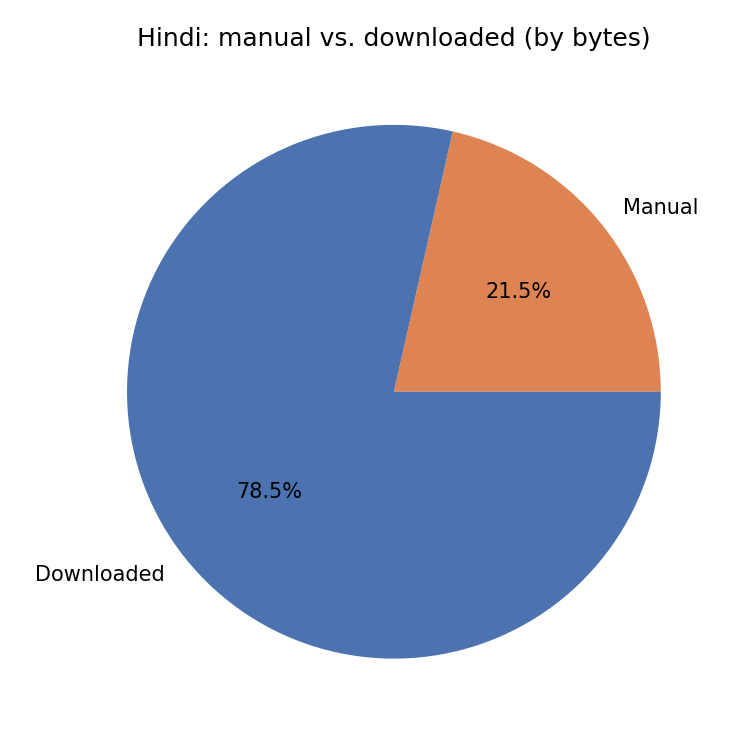
\includegraphics[width=0.32\textwidth]{../phase1/plots/manual_vs_downloaded_hindi.png}
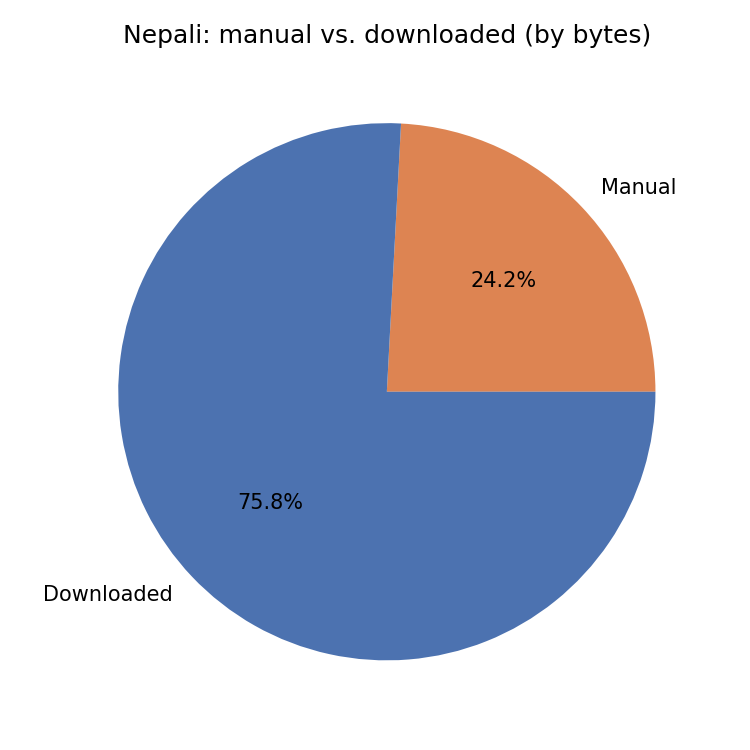
\includegraphics[width=0.32\textwidth]{../phase1/plots/manual_vs_downloaded_nepali.png}
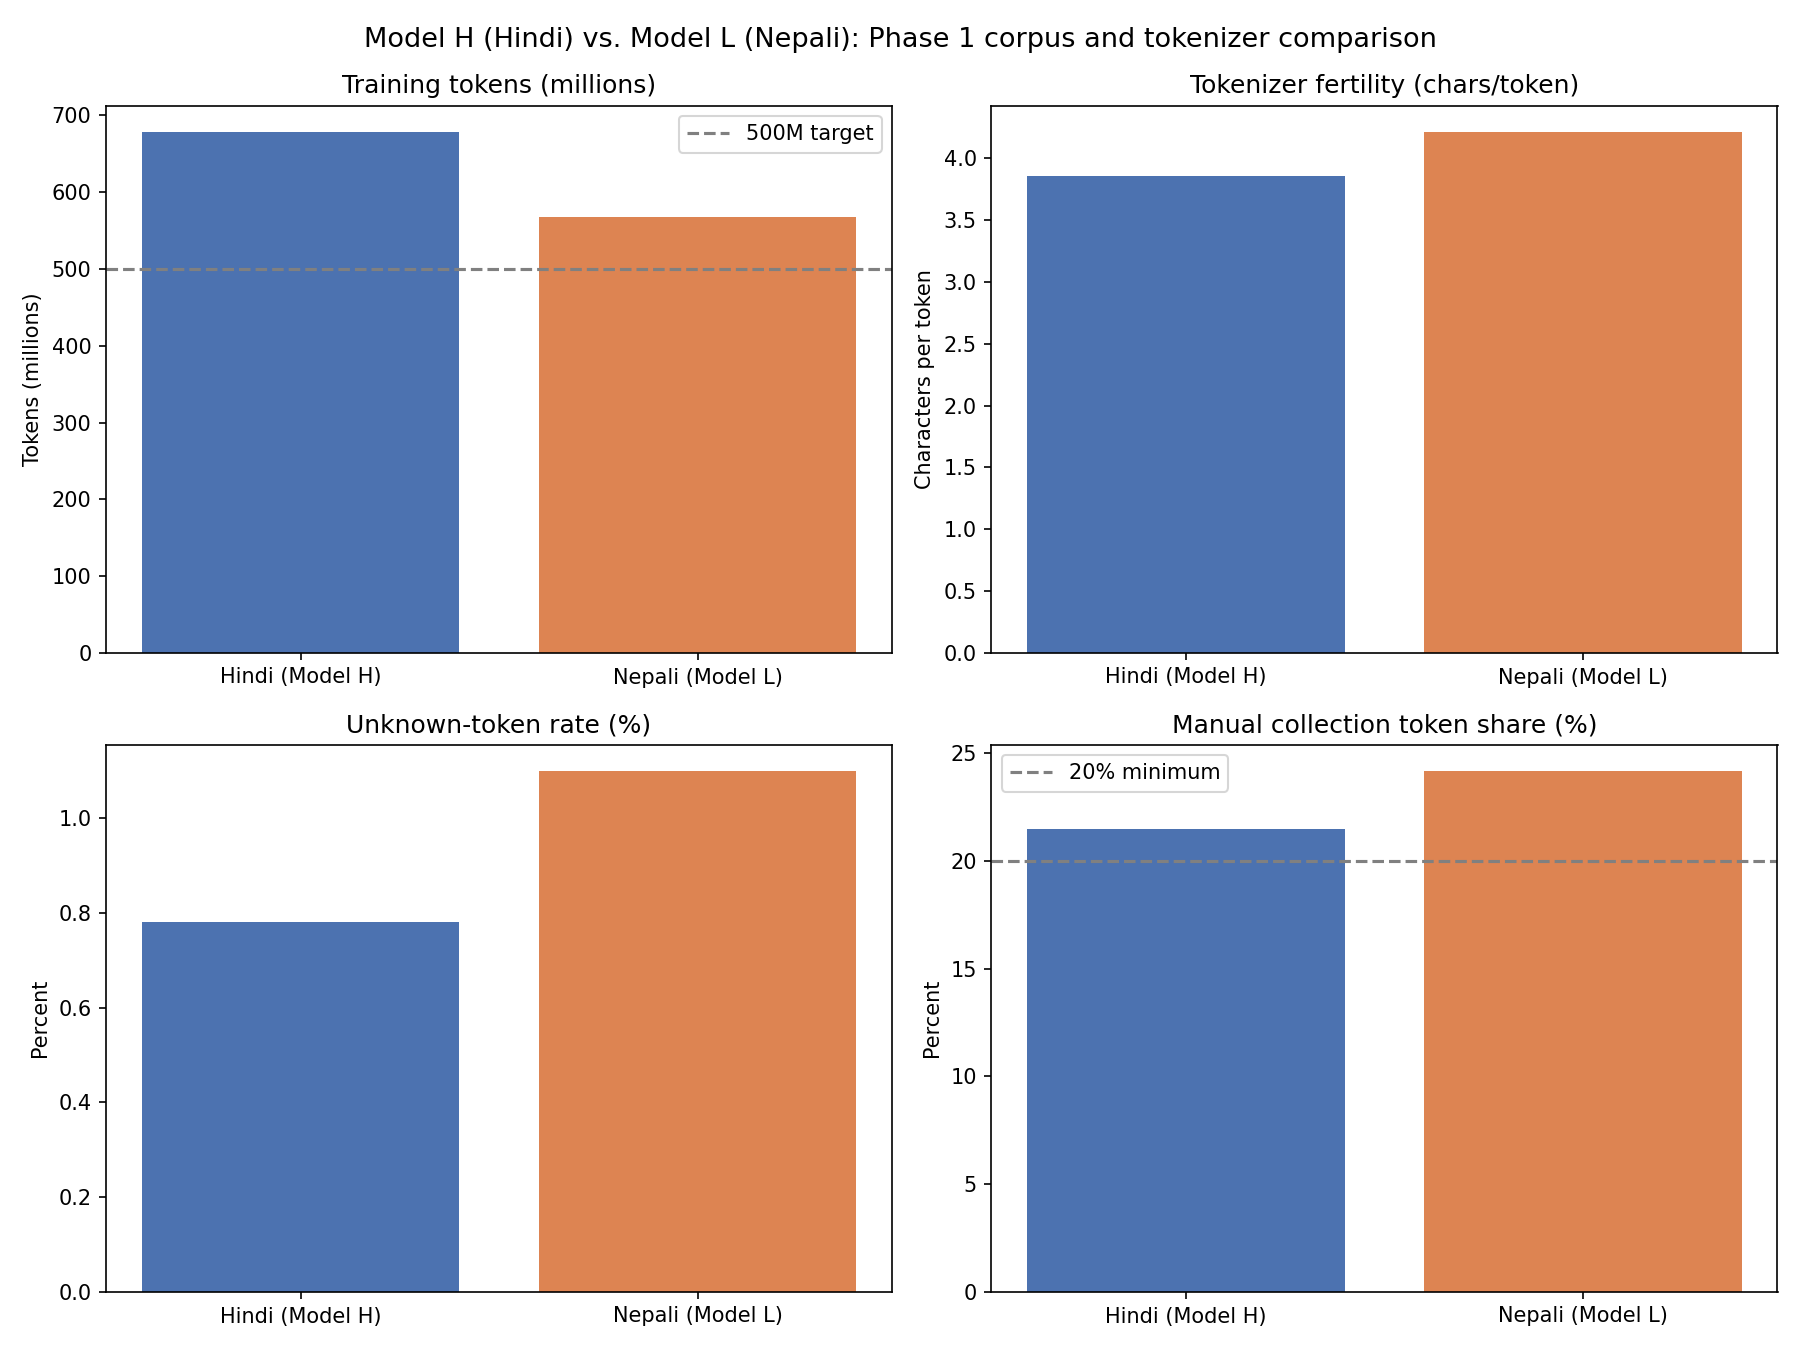
\includegraphics[width=0.32\textwidth]{../phase1/plots/model_h_vs_model_l.png}
\caption{Manual vs. downloaded token share (Hindi, Nepali) and the Phase 1 Model H vs. Model L summary.}
\end{figure}

\section{Phase 2: Architecture, Pretraining, and Evaluation}

\subsection{Architecture}

I wrote a decoder-only Transformer from scratch in PyTorch, using only the basic building blocks (\texttt{nn.Linear}, \texttt{nn.Embedding}, \texttt{nn.LayerNorm}, \texttt{nn.Dropout}). No \texttt{nn.Transformer*}, no HuggingFace anywhere. Same architecture for both models:

\begin{table}[h]
\centering
\small
\begin{tabular}{lr}
\toprule
Model dimension ($d_{model}$) & 384 \\
Layers & 13 \\
Attention heads & 6 (head dimension 64) \\
Feed-forward dimension & 1536 \\
Max sequence length & 256 \\
Parameters (exact, both models) & 26,524,800 \\
\bottomrule
\end{tabular}
\caption{Architecture hyperparameters, identical for Model H and Model L.}
\end{table}

For position, I used RoPE (Rotary Position Embeddings) instead of a learned or sinusoidal scheme. RoPE rotates the query and key vectors inside each attention layer by an angle based on their position. Because of the math behind rotation, the dot product between a query at position $i$ and a key at position $j$ ends up depending only on how far apart they are, $(i-j)$, not on their exact positions. That comes automatically from the rotation, nothing needs to be learned for it. It also adds zero extra parameters, which mattered given the 25M budget. The downside is that RoPE's rotation table only goes up to \texttt{max\_seq\_len = 256}. Beyond that the model has no defined position at all, so 256 tokens is a hard limit on context length, not just a target I chose.

I picked 13 layers instead of a shallower, wider model mainly because Phase 3 needed multi-hop comparisons, chaining $A > B$ and $B > C$ into $A > C$. More layers felt like a better fit for that kind of step-by-step reasoning than extra width would be. I used pre-norm ($x = x + \text{Sublayer}(\text{LayerNorm}(x))$) instead of post-norm, since at 13 layers it keeps the gradient flowing more cleanly through the network during training. I also tied the output layer's weights to the input embedding weights, which alone saves about 3.46M parameters, around 13\% of the whole model.

I tested the causal mask myself instead of just trusting the code. I changed the last token of an input and checked that the logits at every earlier position stayed exactly the same. They did, which confirms the model really cannot see into the future. This check matters more than it sounds like it should. A broken causal mask doesn't crash the program and doesn't obviously show up as a bad loss curve either. The model would just quietly cheat during training by looking ahead at tokens it isn't supposed to see yet, and the loss would look better than it should, right up until you tried to actually generate text one token at a time, where that shortcut no longer exists. Running this test directly, instead of just assuming the code was correct, was worth the few minutes it took.

\subsection{Pretraining}

Both models trained with AdamW, 1,000 steps of linear warmup then cosine decay, batch size 32, sequence length 256, for the full 61,000 steps, around 500M tokens per language. Checkpoints save the weights, optimizer state, scheduler state, the step number, and the config, all in one file, so training can pick back up after an interruption. That mattered because I was training on Kaggle notebooks with a GPU time limit, not a machine I could just leave running.

Both runs finished all 61,000 steps. Loss for both models started around 8.6 nats per token at step 0. That number is $\ln(9000)$, which is exactly what a freshly-initialized model should give if it's just guessing uniformly over a 9,000-token vocabulary. It's a small check, but a useful one: if the starting loss had been noticeably different, that would have meant something was broken in the loss function or the model setup before training even really began. Hindi's loss stayed lower than Nepali's the whole way through training, roughly 3.1 to 3.3 nats per token for Hindi against 3.4 to 3.5 for Nepali. The gap was already there early on, not something that only showed up near the end. That timing matters for the explanation later in this report. If the gap had only shown up late in training, that would point to something like overfitting. Showing up early instead points more toward a difference in the data itself.

\begin{figure}[h]
\centering
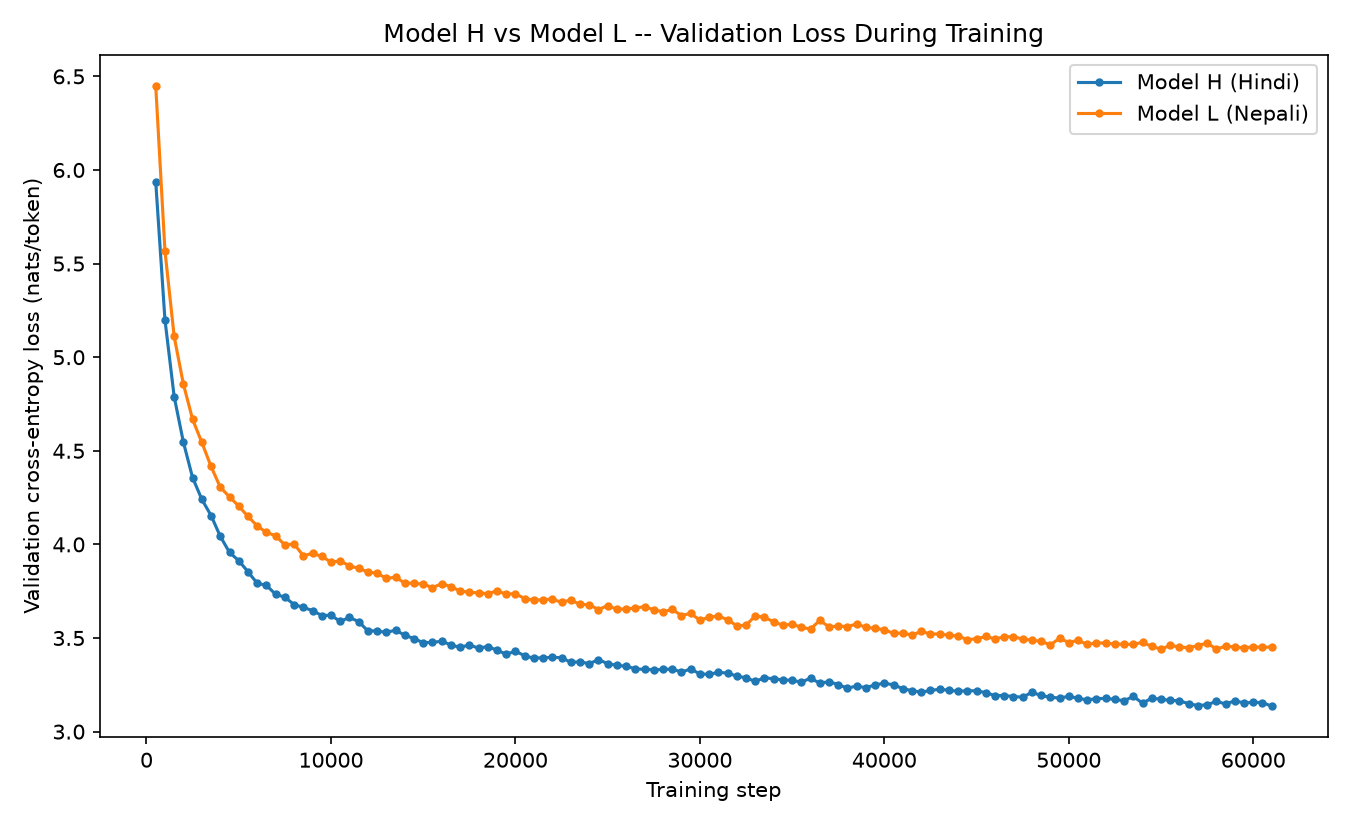
\includegraphics[width=0.32\textwidth]{../phase2/comparison/val_loss_hindi_vs_nepali.png}
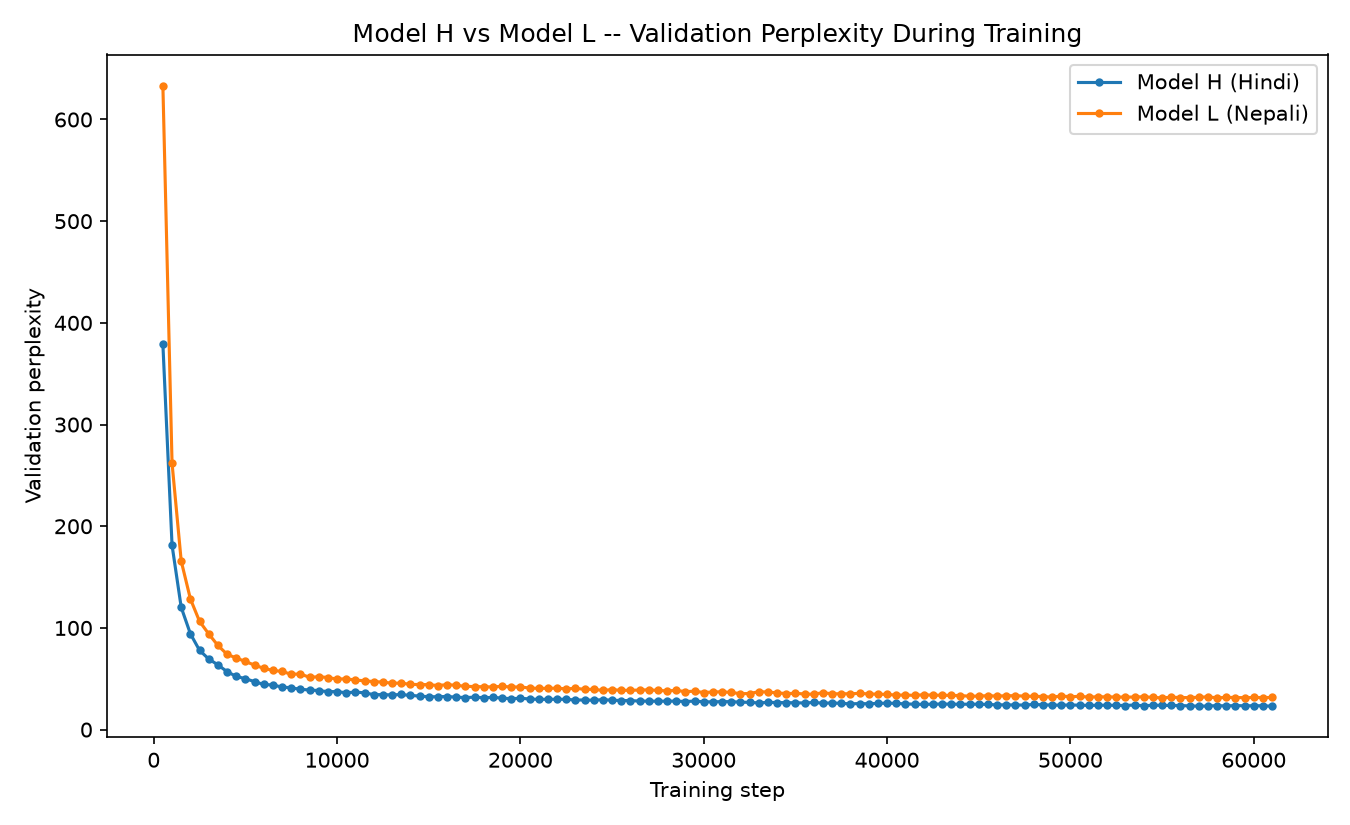
\includegraphics[width=0.32\textwidth]{../phase2/comparison/val_ppl_hindi_vs_nepali.png}
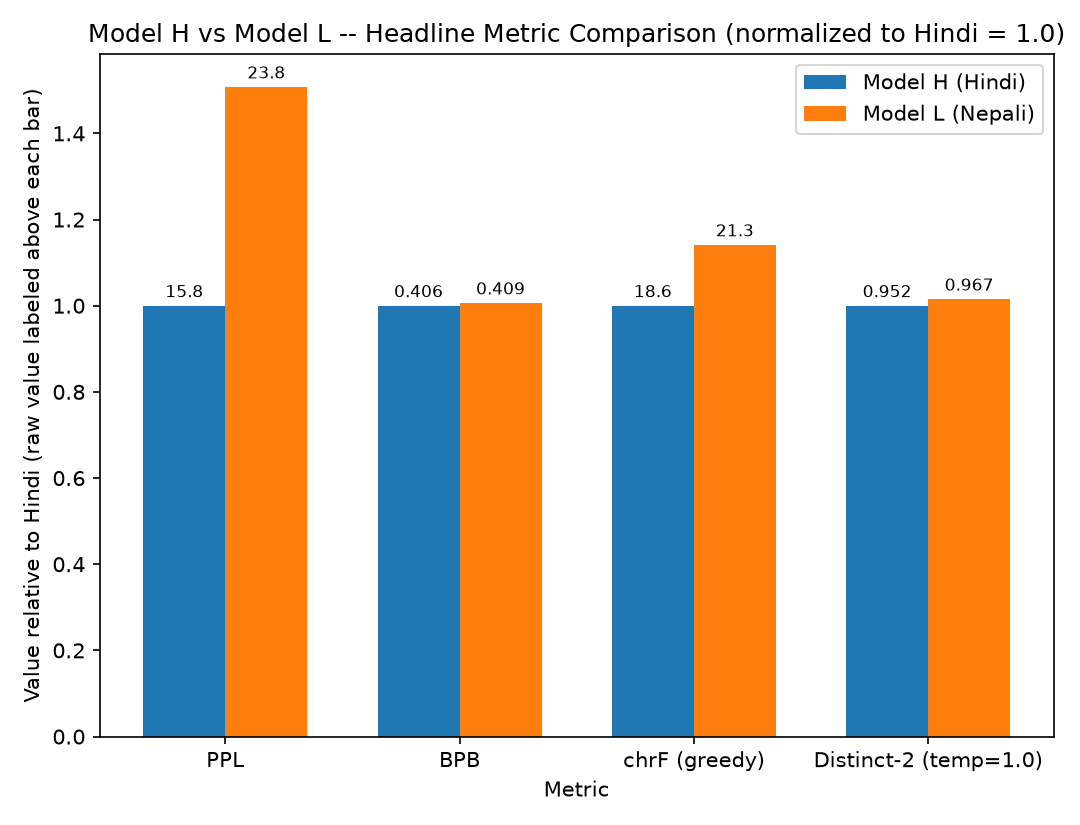
\includegraphics[width=0.32\textwidth]{../phase2/comparison/headline_metrics_bar.png}
\caption{Validation loss, validation perplexity (both overlaid, Hindi vs. Nepali), and headline metrics comparison.}
\end{figure}

\begin{figure}[h]
\centering
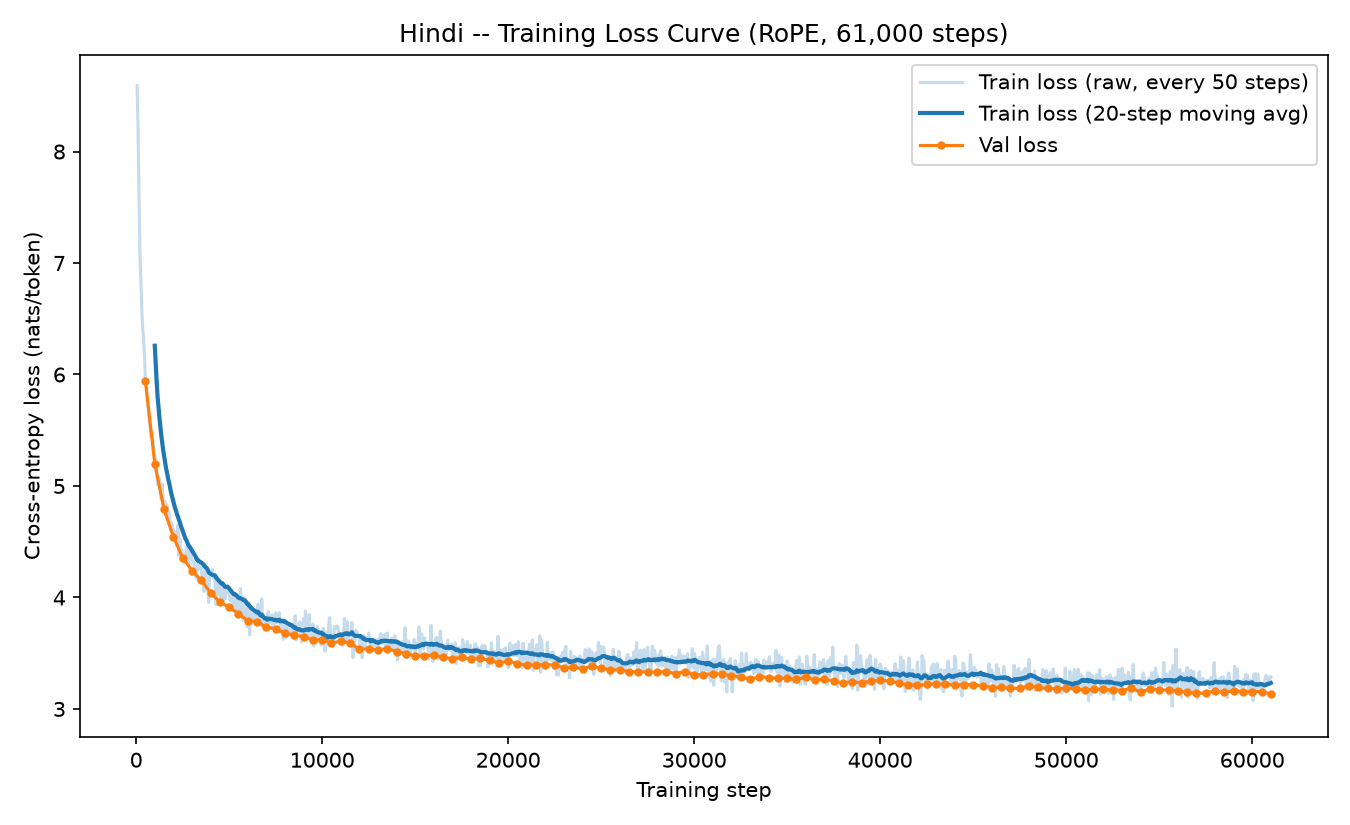
\includegraphics[width=0.32\textwidth]{../phase2/hindi/plots/training_loss_curve.png}
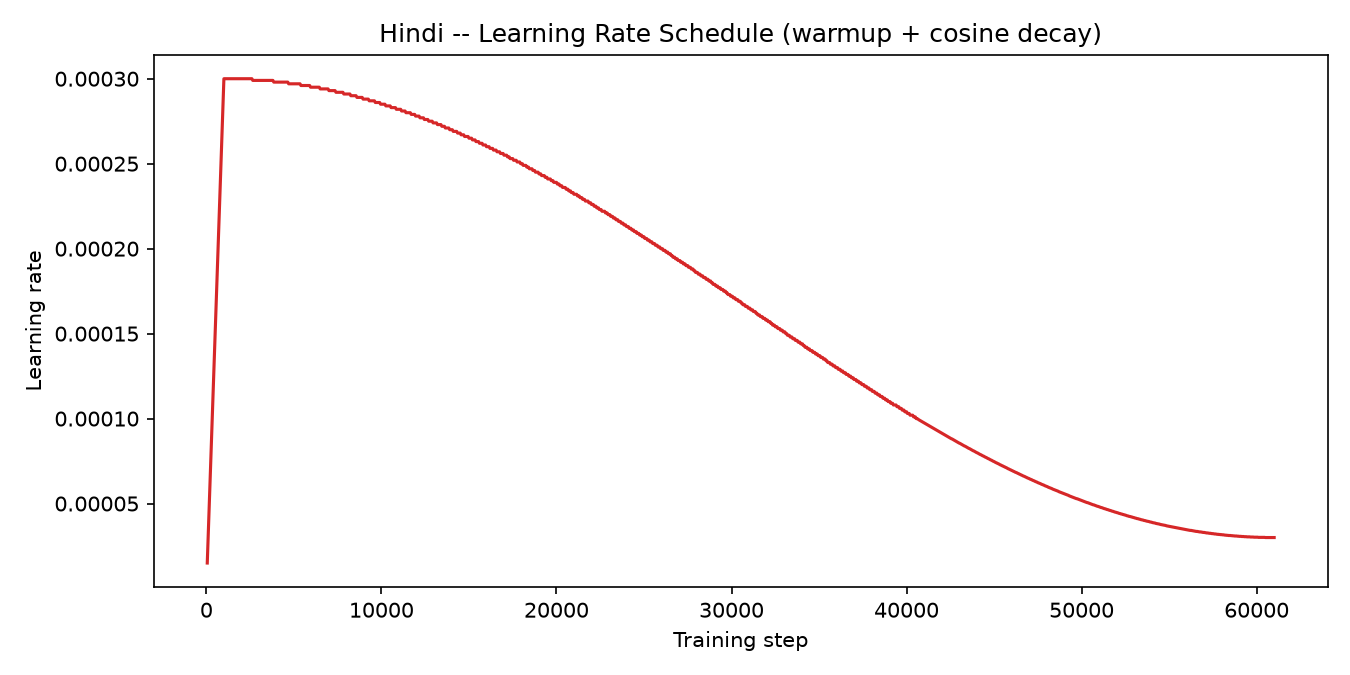
\includegraphics[width=0.32\textwidth]{../phase2/hindi/plots/lr_schedule.png}
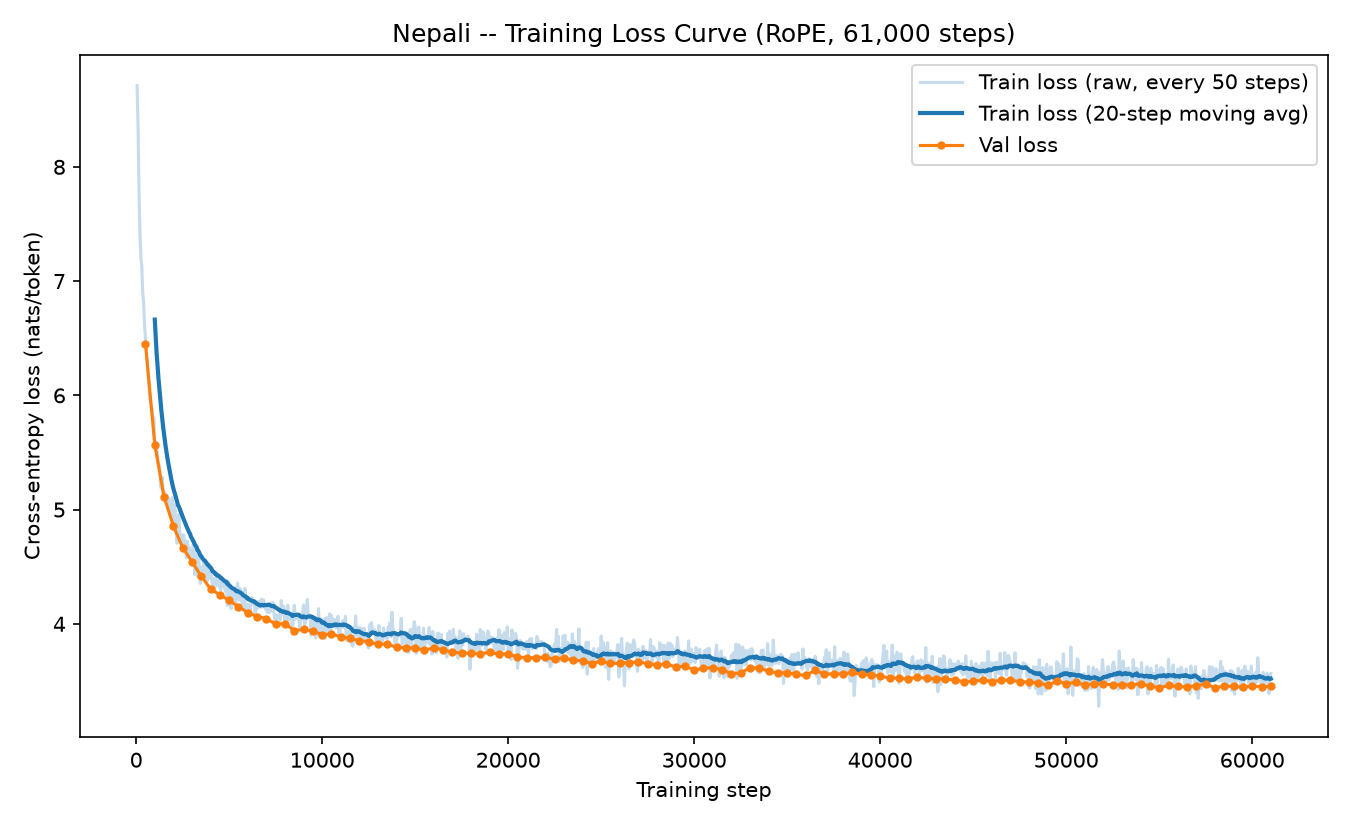
\includegraphics[width=0.32\textwidth]{../phase2/nepali/plots/training_loss_curve.png}
\caption{Hindi training loss curve, Hindi LR schedule (Nepali's schedule has the same shape), and Nepali training loss curve.}
\end{figure}

\subsection{Perplexity and bits-per-byte}

\begin{table}[h]
\centering
\small
\begin{tabular}{lrr}
\toprule
 & Hindi (Model H) & Nepali (Model L) \\
\midrule
Perplexity (test set) & 15.77 & 23.78 \\
Bits-per-byte (test set) & 0.4063 & 0.4089 \\
\bottomrule
\end{tabular}
\caption{Perplexity and bits-per-byte, both models, on their own held-out test splits.}
\end{table}

The perplexity gap looks big: 23.78 for Nepali against 15.77 for Hindi, about 50\% higher. But the bits-per-byte gap is tiny: 0.4089 vs 0.4063, under 1\% apart. Here is why. Perplexity is measured per token, and the two models use two different tokenizers. Nepali's tokenizer makes more tokens per character (fertility 4.22 vs 3.86), so the same piece of Nepali text turns into more prediction steps than the same piece of Hindi text. More steps means a bigger perplexity number, even if the model isn't actually worse at understanding the language. Bits-per-byte counts raw bytes instead of tokens, so it doesn't care how the tokenizer chops the text up. That makes it the fairer number, and it says the two models are much closer than perplexity alone makes them look.

\subsection{Generation quality and diversity}

I generated continuations from held-out prompts with greedy decoding and temperatures 0.5, 1.0, and 1.5, then scored them against the real continuation with BLEU, chrF, and ROUGE-L, plus repetition rate and Distinct-1/Distinct-2 for diversity.

\begin{table}[h]
\centering
\small
\begin{tabular}{llrrrrrr}
\toprule
Model & Condition & BLEU & chrF & ROUGE-L & Distinct-1 & Distinct-2 & Repetition rate \\
\midrule
Hindi & Greedy & 1.67 & 18.63 & 0.020 & 0.270 & 0.460 & 0.75 \\
Hindi & T=0.5 & 3.06 & 21.04 & 0.000 & 0.388 & 0.759 & 0.60 \\
Hindi & T=1.0 & 0.86 & 20.65 & 0.011 & 0.603 & 0.952 & 0.05 \\
Hindi & T=1.5 & 0.25 & 18.78 & 0.000 & 0.831 & 1.000 & 0.00 \\
\addlinespace
Nepali & Greedy & 2.92 & 21.26 & 0.000 & 0.324 & 0.491 & 0.90 \\
Nepali & T=0.5 & 2.03 & 23.07 & 0.000 & 0.455 & 0.702 & 0.70 \\
Nepali & T=1.0 & 0.53 & 21.12 & 0.000 & 0.777 & 0.967 & 0.00 \\
Nepali & T=1.5 & 0.09 & 19.44 & 0.000 & 0.900 & 0.999 & 0.00 \\
\bottomrule
\end{tabular}
\caption{Generation quality, all four decoding conditions, both models.}
\end{table}

BLEU stays low the whole time, never above about 3 out of 100 for either language. I don't read much into that, since BLEU is comparing one open-ended generated continuation against one single fixed reference, and there are plenty of reasonable ways to continue a news article that would still score near zero against that one reference. chrF compares character-level patterns instead of whole words, and it sits higher and steadier. That fits with both languages having a lot of inflection, since character overlap still picks up similar word forms even when BLEU's whole-word matching misses them completely. The part that actually tells us something is the tradeoff between repetition and diversity as temperature goes up. Under greedy decoding, both models repeat themselves a lot: 75\% of Hindi outputs and 90\% of Nepali outputs contain a repeated four-word sequence, and diversity is low. By temperature 1.0, repetition drops to almost nothing and Distinct-2 climbs past 0.95 for both languages. Since this pattern shows up almost the same way in both languages, it looks like something small models do under greedy decoding in general, not something specific to either language.

\subsection{Attention analysis}

I looked at attention entropy, which measures how spread out each head's attention is, and mean attention distance, which measures how far back each head usually looks, across all layers, for both models. In both languages, each head tends to settle into one of two roles: a "local" head with short distance and low entropy, or a "long-range" head with high entropy and large distance. A head mostly keeps its role as you go deeper into the network, it doesn't switch back and forth. Since RoPE gives every layer fresh position information, not just the first one, a head in a late layer that attends broadly over content is doing that on purpose, not because position information has run out by then.

\begin{figure}[h]
\centering
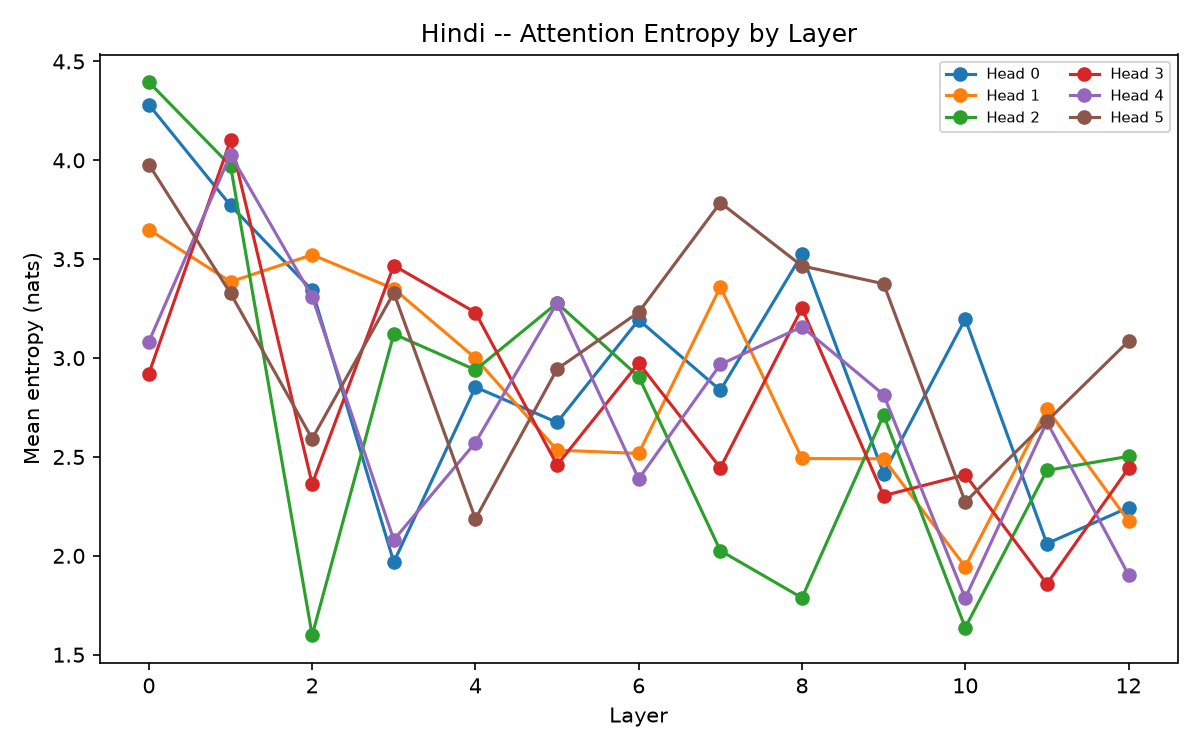
\includegraphics[width=0.32\textwidth]{../phase2/hindi/plots/attention_entropy_by_layer.png}
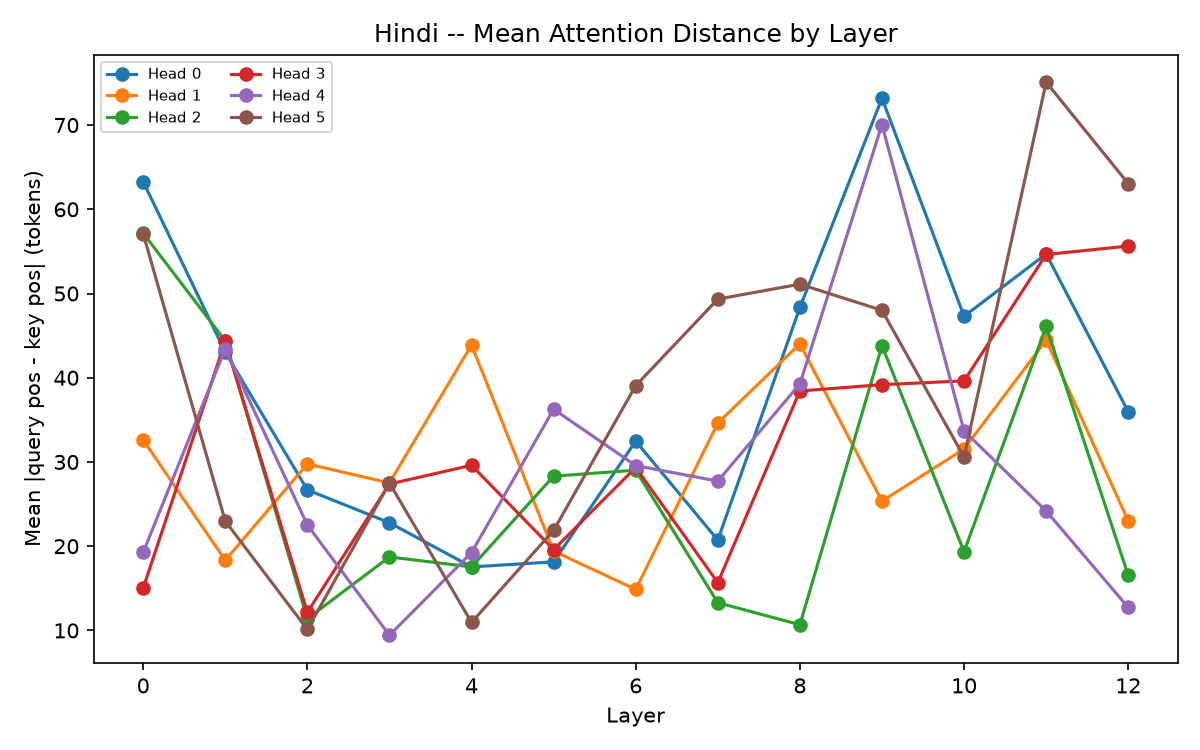
\includegraphics[width=0.32\textwidth]{../phase2/hindi/plots/attention_distance_by_layer.png}
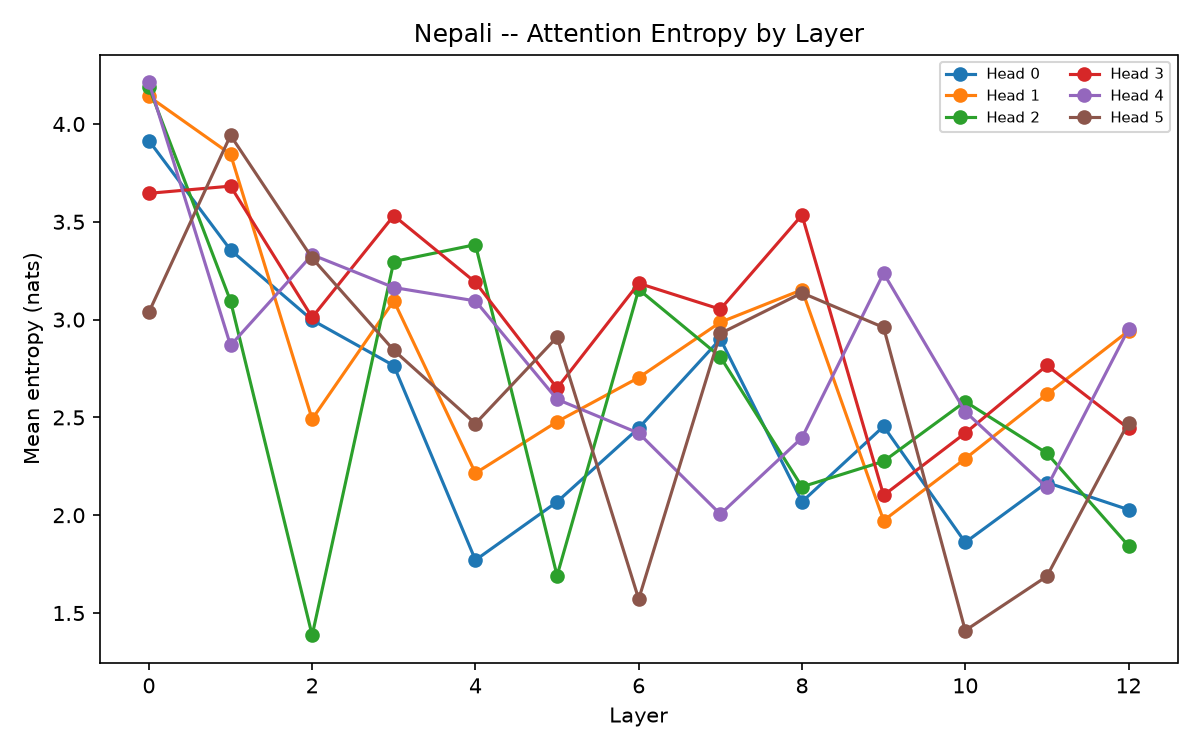
\includegraphics[width=0.32\textwidth]{../phase2/nepali/plots/attention_entropy_by_layer.png}
\caption{Attention entropy and mean distance by layer: Hindi entropy, Hindi distance, Nepali entropy (Nepali's distance-by-layer plot shows the same qualitative pattern).}
\end{figure}

I also looked at the actual attention heatmaps, which show query position against key position for every head, at the earliest and latest layer, for both models. These are left out of this PDF to stay under the page limit, but the full set is under \path{report/phase2/hindi/plots/} and \path{report/phase2/nepali/plots/}. At layer 0, both languages show several heads with a clear diagonal band, meaning they mostly attend to the few tokens right before the current one. By the last layer, some heads keep that local pattern while others spread out over many earlier positions, which matches the entropy and distance numbers above. The two languages look similar here. I didn't find any head pattern in one language that was simply missing in the other.

\subsection{Why Hindi and Nepali differ at this stage}

Both languages use the same script and the same vocabulary size, so those two things aren't causing the gap. What is different is how much training data each language has. Hindi has about 111 million more tokens than Nepali, 679M against 568M, roughly 19\% more. That's mostly because Hindi has more large, active news sites and a bigger Wikipedia to pull from. Nepali's tokenizer also has slightly worse fertility (4.22 vs 3.86). If anything that should make next-token prediction a little easier for Nepali, not harder, since worse fertility means more characters packed into each token. So the fact that Nepali still does worse on loss and bits-per-byte makes me fairly confident the real cause is the token-count gap, not some tokenizer side effect.

\section{Phase 3: Reasoning Finetuning and Attention Comparison}

\subsection{Synthetic reasoning dataset}

I built my own comparative-reasoning dataset for each language instead of downloading one, so I'd actually know the correct answer for every example. Each example gives two or three people a numeric attribute (height, age, price, weight, or distance) and asks a comparison question, in three shapes: pairwise (compare two people directly), ranking (pick the largest or smallest of three), and transitive (three people listed in decreasing order, but only the two neighboring relationships are stated out loud, so the model has to chain through the middle person to answer about the two whose relationship was never stated directly). Everything is written in the language itself, in Devanagari script, with names drawn from separate pools per language. Nothing is translated from English.

To stop the model from just memorizing the test set, I held back about a quarter of each language's name pool so those names only ever show up in validation or test, never training, and I held back one whole attribute (distance) from training entirely so it only appears in val/test. I wrote automated tests that check these two things every time the dataset gets regenerated.

\begin{table}[h]
\centering
\small
\begin{tabular}{lrr}
\toprule
 & Hindi & Nepali \\
\midrule
Train examples & 6,000 & 6,000 \\
Validation examples & 600 & 600 \\
Test examples & 800 & 800 \\
\bottomrule
\end{tabular}
\caption{Reasoning dataset sizes, both languages.}
\end{table}

Within the test set, the three question types aren't split evenly: transitive questions make up roughly 40\% of test/validation but only about 20\% of train, since chaining through a middle person is the harder skill and I wanted more of the harder cases in evaluation. Pairwise and ranking split the rest of each set fairly evenly.

\subsection{Finetuning}

I finetuned each model starting from its own Phase 2 pretrained checkpoint, with that language's tokenizer completely frozen. Loss is only computed on the answer tokens, not on the facts or the question part, so the model isn't penalized for how it represents the question itself. I used a lower learning rate than pretraining (5e-5 instead of 3e-4), since this is a short run on a small dataset (6,000 examples) and I didn't want to wreck what the model already knew about the language.

Hindi's validation loss was lowest at epoch 6, Nepali's at epoch 7. Neither is the last epoch, so I used the best checkpoint by validation loss, not the final one, for everything below.

\begin{figure}[h]
\centering
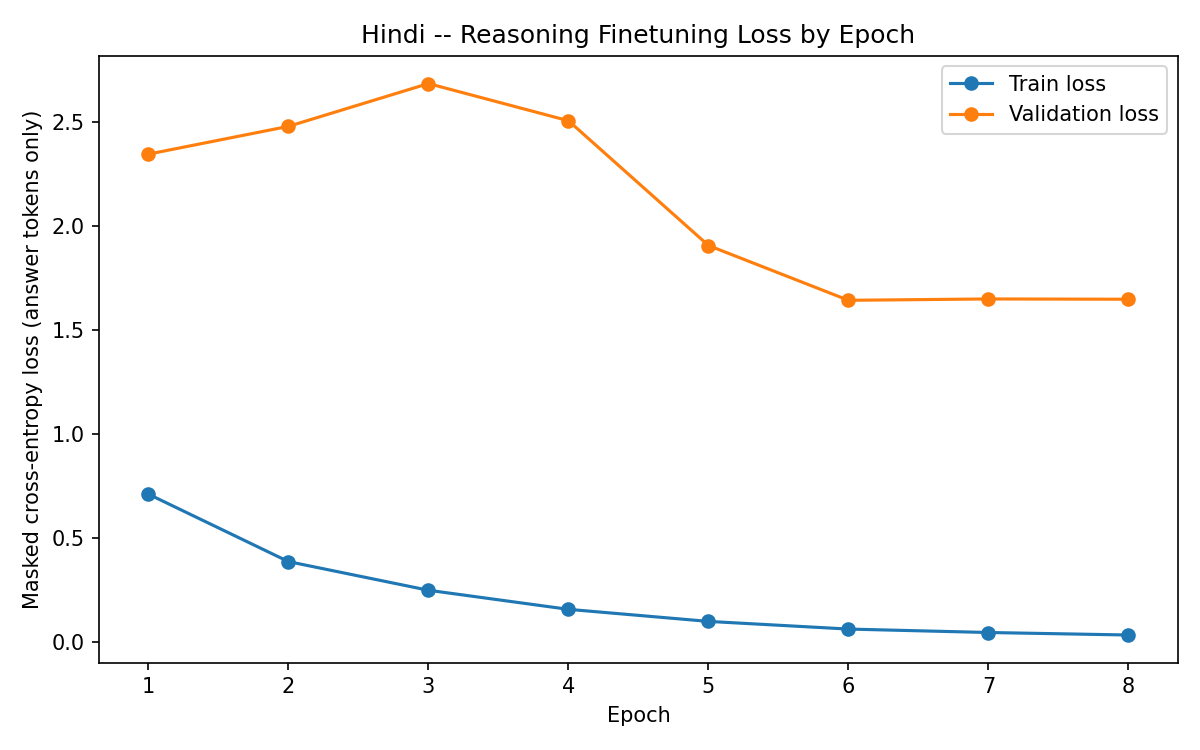
\includegraphics[width=0.48\textwidth]{../phase3/hindi/plots/finetune_loss_curve.png}
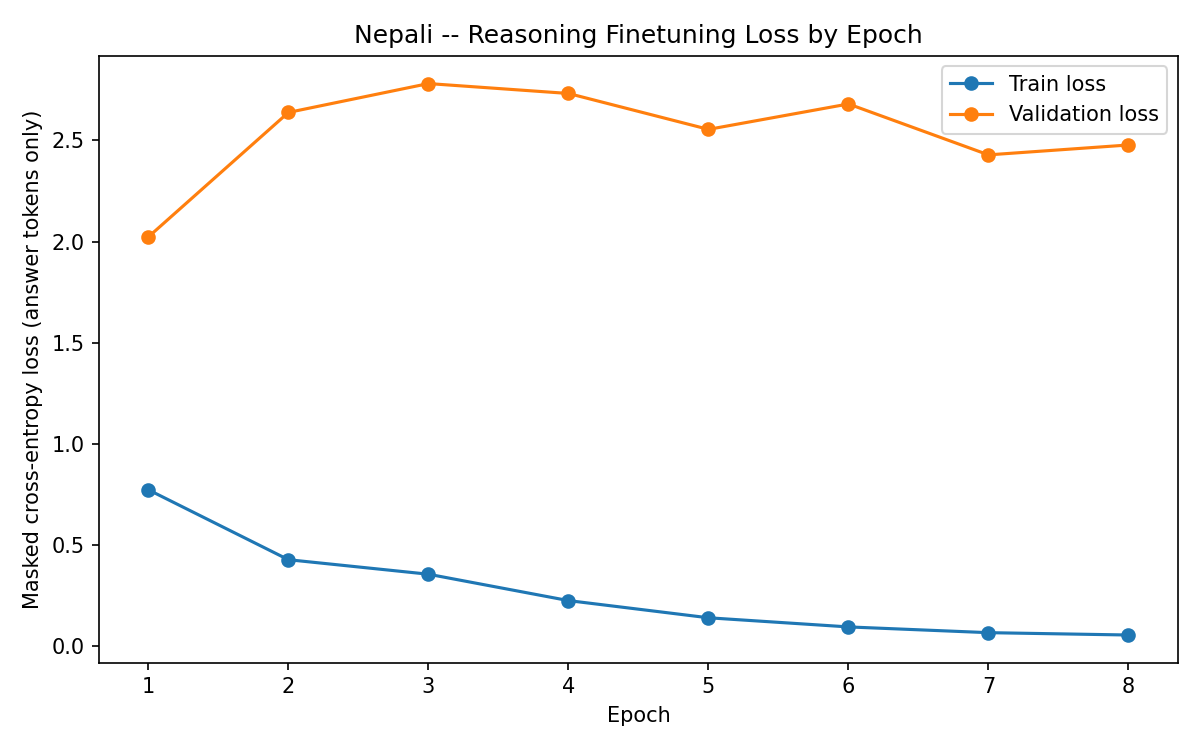
\includegraphics[width=0.48\textwidth]{../phase3/nepali/plots/finetune_loss_curve.png}
\caption{Reasoning finetuning loss curve, Hindi (left) and Nepali (right).}
\end{figure}

\subsection{Pretrained vs finetuned accuracy}

\begin{table}[h]
\centering
\small
\begin{tabular}{lrr}
\toprule
 & Hindi (Model H) & Nepali (Model L) \\
\midrule
Pretrained accuracy & 0.0\% & 0.0\% \\
Finetuned accuracy (overall) & 47.1\% & 40.1\% \\
\ \ Pairwise & 20.3\% & 13.8\% \\
\ \ Ranking & 18.6\% & 11.3\% \\
\ \ Transitive & 86.1\% & 82.8\% \\
\bottomrule
\end{tabular}
\caption{Reasoning accuracy before and after finetuning, both languages.}
\end{table}

Before finetuning, both models score exactly 0\%. That's not surprising, since they've never seen this question format before and have no reason to answer with a name at all. But this 0\% baseline is still useful to have: it means every point of the 47.1\%/40.1\% finetuned accuracy is something the model actually learned during the reasoning finetune, not something it could already sort of do from pretraining. After finetuning, both models improve a lot, with Hindi about 7 points ahead overall. The fact that this gap carries over from Phase 2 into Phase 3, in the same direction, tells me something too: whatever separates the two models isn't limited to plain language modeling. It shows up again in a task that's specifically about reasoning over facts, not just predicting natural text.

The bigger surprise isn't the Hindi/Nepali gap, it's the gap between question types. Transitive questions score 82--86\% for both languages, but pairwise and ranking only reach 11--20\%. At first this looks like the models are unusually good at the "hard" multi-hop question type. But when I looked back at how I built the dataset, I found a simpler explanation. Every transitive question names the three people in decreasing order and always asks about the first-named person versus the last-named one. So a model can score well on transitive questions just by learning "the first name mentioned is usually the answer," without actually chaining through the middle person at all. Pairwise and ranking questions don't give it that shortcut, since the right answer can be in any position. So I think the 11--20\% scores on those two types are a more honest measure of how well the models actually learned to compare things. When I looked at the wrong pairwise and ranking answers, the model often named someone who wasn't even mentioned in the question. That looks more like a formatting mistake than a real reasoning failure.

\begin{table}[h]
\centering
\small
\begin{tabular}{lll}
\toprule
Question type & Expected answer & Hindi model's answer \\
\midrule
Transitive & Correct name & Correct (match) \\
Transitive & Correct name & Correct (match) \\
Pairwise & One of the two named people & A name not in the question (wrong) \\
Ranking & One of the three named people & A name not in the question (wrong) \\
\bottomrule
\end{tabular}
\caption{Pattern in Hindi finetuned model's reasoning outputs, from the actual evaluation run. Both wrong answers named someone who wasn't even one of the choices offered.}
\end{table}

\subsection{Attention before and after finetuning}

I reused the same attention-analysis code from Phase 2 on the finetuned checkpoints, just pointed it at reasoning prompts instead of news text. The early layers, layer 0 and roughly layers 1--2, barely move after finetuning: entropy at layer 0 shifts by less than 0.02 nats for both languages. The middle layers change the most. For Hindi, layer 5's entropy drops by about 0.52 nats after finetuning, the biggest change anywhere in the network, and Nepali shows the same pattern, with its own biggest drop also around layer 5. Mean attention distance drops in those same middle layers too. Hindi's layer 5 goes from attending about 6.6 tokens back on average to about 4.7.

\begin{figure}[h]
\centering
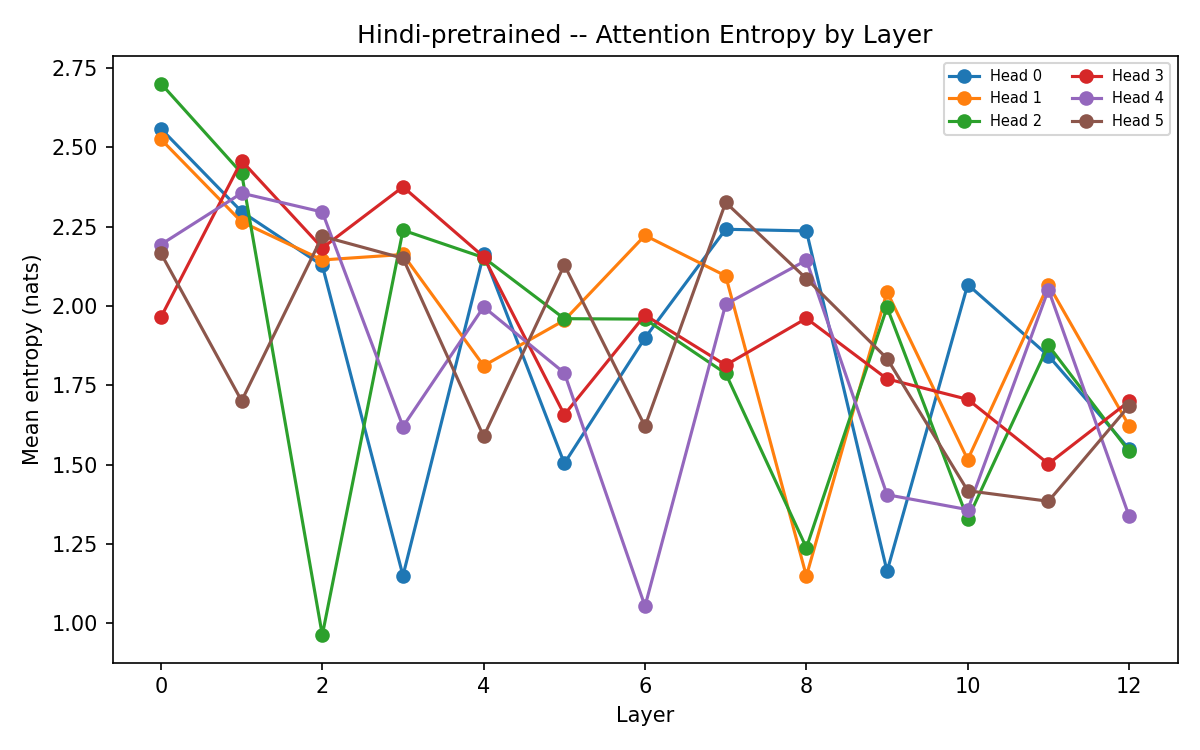
\includegraphics[width=0.32\textwidth]{../phase3/hindi/plots/attention_entropy_by_layer_pretrained.png}
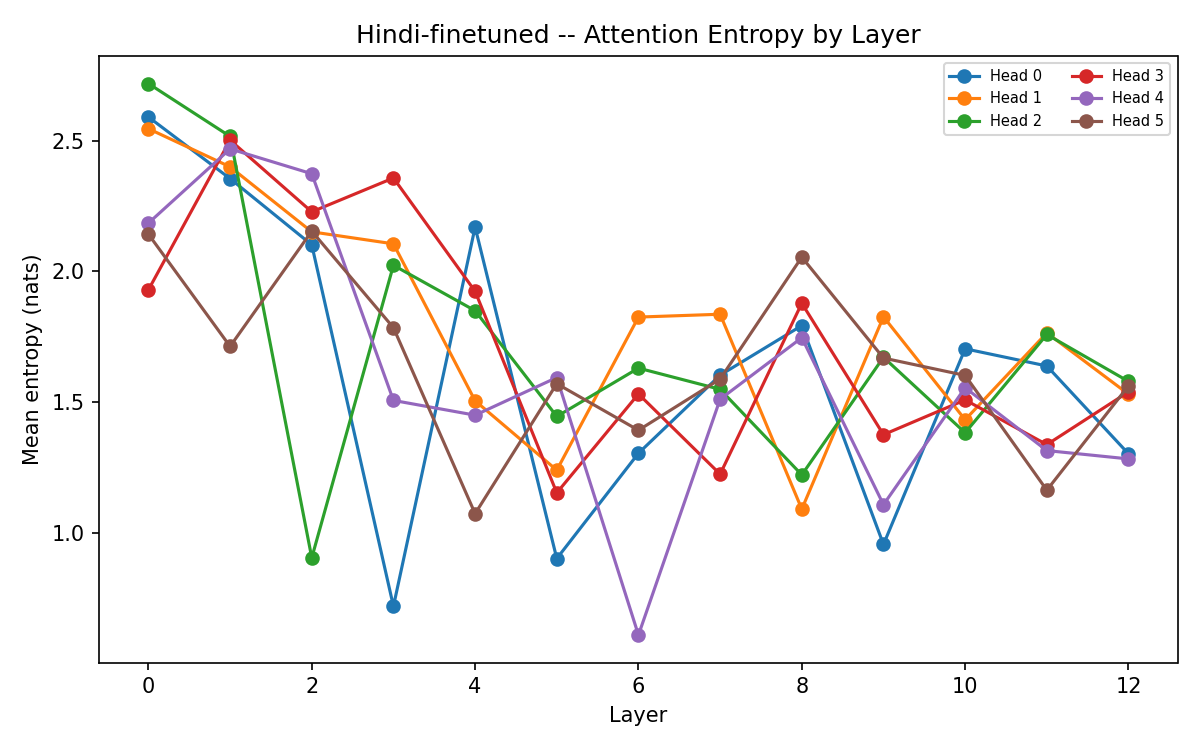
\includegraphics[width=0.32\textwidth]{../phase3/hindi/plots/attention_entropy_by_layer_finetuned.png}
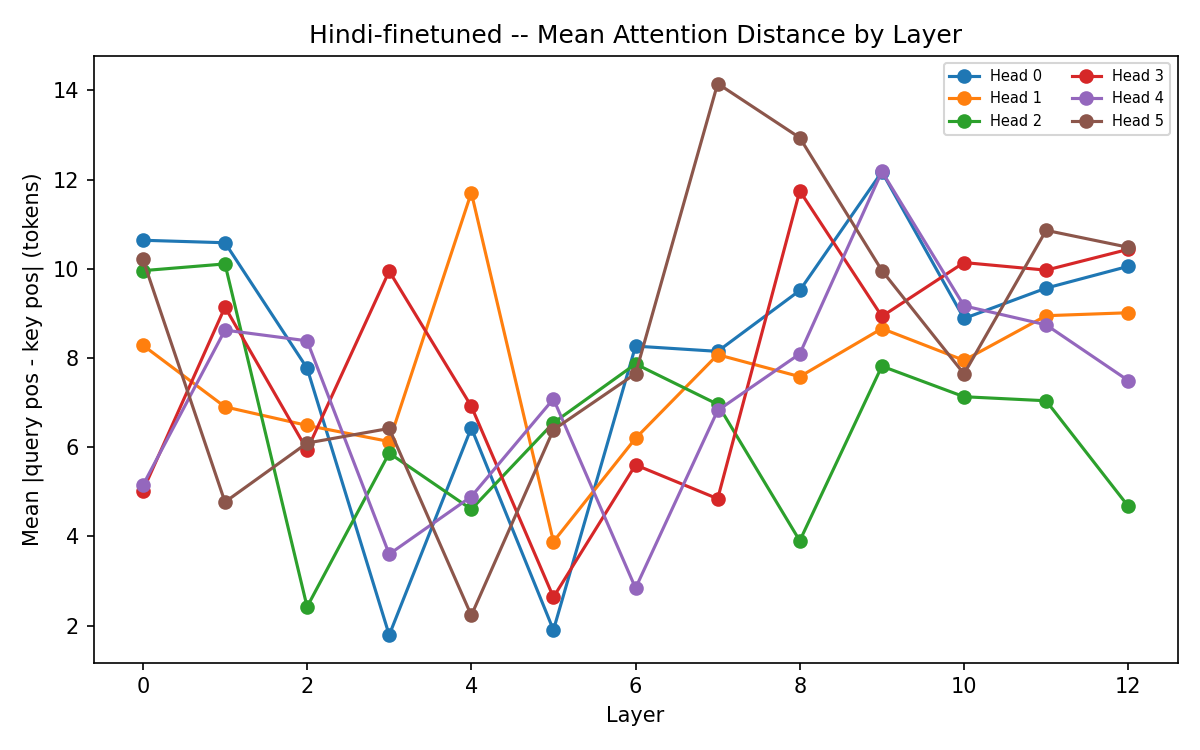
\includegraphics[width=0.32\textwidth]{../phase3/hindi/plots/attention_distance_by_layer_finetuned.png}
\caption{Hindi attention entropy, pretrained vs. finetuned, and finetuned mean attention distance by layer (Nepali shows the same qualitative pattern; see \texttt{report/phase3/nepali/plots/}).}
\end{figure}

I also checked the actual heatmaps, left out of this PDF for space, with the full set under \path{report/phase3/hindi/plots/} and \path{report/phase3/nepali/plots/}. Layer 0 looks almost the same before and after finetuning for both languages, still a clear diagonal band. The last layer looks genuinely different. Before finetuning, attention is spread across several points. After finetuning, several heads collapse onto one strong vertical stripe at a single key position, and in the examples I checked, that position lines up with where the first person's number appears in the prompt. My read on this is that those heads learned to lock onto the specific number they need to compare against, once the model had a concrete task to do, instead of spreading attention more broadly the way it does over open-ended news text.

\subsection{Final comparison across all three phases}

Putting all three phases side by side, Hindi comes out ahead of Nepali at every stage, but never by a huge margin. It's a small, repeated edge rather than one big gap. Below I answer the four questions this final report is supposed to cover directly.

\paragraph{1. How did data scale and quality differ between Model H and Model L?}
Hindi ended up with about 19\% more pretraining tokens than Nepali, 679M against 568M. Both cleared the assignment's ~500M-token target and the 20\% manual-collection minimum, so this isn't a case of Nepali falling short of the requirements, just having less to work with overall. The quality difference shows up mainly in the tokenizer: at the same 9,000-token vocabulary size, Hindi gets better fertility (3.86 vs 4.22 characters per token) and a lower unknown-token rate (0.78\% vs 1.10\%). Both corpora went through identical cleaning steps and are confirmed to share zero documents with each other, so the gap is about how much clean, usable text each language had, not about one corpus being messier than the other.

\paragraph{2. How do language-modeling and reasoning results compare across the two resource tiers?}
Hindi is ahead at every stage. But how big the gap looks depends a lot on which metric you check. Perplexity makes it look large: 23.78 for Nepali against 15.77 for Hindi, about 50\% higher. Bits-per-byte isn't affected by tokenizer differences, and it tells a much closer story: 0.4089 vs 0.4063, under 1\% apart. That same gap carries into Phase 3. Hindi's finetuned reasoning accuracy is 47.1\% against Nepali's 40.1\%, a 7-point gap in the same direction as the language-modeling gap. So Hindi's advantage is real and it's consistent, but it's modest. This isn't one model working and the other failing.

\paragraph{3. What tokenizer / corpus factors most affected the lower-resource model?}
Two factors matter here, and they point in opposite directions. The main one is Nepali's smaller token count, 568M against 679M. This lines up with Nepali's worse loss and worse bits-per-byte all through training. Nepali's tokenizer fertility is also worse, 4.22 characters per token against 3.86 for Hindi. But this should actually help Nepali, not hurt it. A worse fertility means each token packs in more characters, so the model has fewer, denser prediction steps to get right. Since Nepali still does worse overall even with that small advantage, the real driver looks like the token-count gap, not the tokenizer.

\paragraph{4. What evidence explains the observed differences?}
Three pieces of evidence, put together. First, the training loss curves show the Hindi/Nepali gap appearing early in training, not just near the end. That points to a difference in the data itself, not something like overfitting late in the run. Second, the bits-per-byte numbers strip out the tokenizer's effect and still show Hindi ahead, so fertility isn't the main explanation. Third, the reasoning-accuracy gap in Phase 3 moves in the same direction as the Phase 2 language-modeling gap, even though the finetuning setup itself, meaning dataset size, hyperparameters, and epochs, was identical for both languages. Taken together, this points to Nepali entering Phase 3 with a slightly weaker pretrained checkpoint, and that small disadvantage carrying through finetuning, rather than the reasoning task itself treating the two languages differently. Both languages share a script and both had real news sites and a real Wikipedia to draw from. So I'd expect a genuinely lower-resource language from the assignment's list, one with far fewer public sources than Nepali has, to show a bigger version of this same pattern.

\section{Limitations}

A few things I'd flag rather than gloss over. Sample sizes for generation quality are small: 20 prompts per language, scored against a single reference each, which is why I don't put much weight on the BLEU/ROUGE-L numbers beyond the general repetition-vs-diversity trend. The reasoning dataset's transitive-question format has the first-named-person shortcut described above, so the 86\% Hindi transitive score is probably an overestimate of real chaining ability; a cleaner dataset would randomize which position holds the correct answer. Everything here is a single training run per model, not averaged over multiple seeds, so a small part of the Hindi/Nepali gap could in principle be run-to-run noise, though a roughly 50\% perplexity gap and a consistent 7-point reasoning gap both feel too large to be entirely down to randomness. Both models are also small (26.5M parameters, 500M tokens), so none of these findings should be assumed to hold at a larger scale without checking.

\section{Bonus: no-positional-embeddings ablation}

As an optional extra, I took Model H and trained a second copy of it with positional embeddings removed. In this version the attention layers never call RoPE, so every attention score comes only from the content of the tokens, not their position. The causal mask (which token comes before which) is the only sense of order left in the model. Everything else stayed the same: same architecture, same 679M-token corpus, same tokenizer, same 61,000-step training budget. That way, any difference between the two models has to come from removing position information, not from some other change. Normally RoPE gives every attention head exact information about how far apart two tokens are, for free, without the model having to learn it. Take that away, and the model has to spend some of its limited capacity trying to guess position from content alone, on top of its normal job of understanding what the words mean. The question I wanted to answer was how much that actually costs, and which parts of the network are affected the most.

\subsection{Perplexity and bits-per-byte}

\begin{table}[h]
\centering
\small
\begin{tabular}{lrrr}
\toprule
 & Standard (RoPE) & Ablated (no position) & Change \\
\midrule
Perplexity (matched test set) & 15.28 & 16.52 & +8.2\% worse \\
Bits-per-byte (matched test set) & 0.4015 & 0.4131 & +2.9\% worse \\
\bottomrule
\end{tabular}
\caption{Standard vs. ablated Hindi model, evaluated on the identical 16,384,000-token test sample so the two numbers are directly comparable.}
\end{table}

An 8\% perplexity hit and a 3\% bits-per-byte hit is a real gap, not noise. Both numbers move the same direction on a large, matched test set. But it is a moderate gap, nowhere near what you would see if the model were guessing almost randomly. This tells me the model can partly work around missing position using two things it still has. First, the causal mask itself carries a small amount of position information: a token near the start of the text has fewer earlier tokens to attend to than a token near the end, and the model can learn to use that as a rough clue. Second, in real text, position and content are already linked. Words that belong together grammatically tend to sit close to each other anyway, so a model that is good at matching related content will often end up attending nearby without being told to. Position information clearly helps, but it isn't the only way to get reasonable predictions.

\subsection{Generation quality and diversity}

\begin{table}[h]
\centering
\small
\begin{tabular}{llrrrr}
\toprule
Model & Condition & Distinct-2 & Repetition rate \\
\midrule
Standard & Greedy & 0.4244 & 0.86 \\
Ablated & Greedy & 0.3746 & 0.94 \\
Standard & T=1.0 & 0.9138 & 0.06 \\
Ablated & T=1.0 & 0.9231 & 0.06 \\
\bottomrule
\end{tabular}
\caption{Generation diversity/repetition, standard vs. ablated Hindi model, matched conditions (50 samples each).}
\end{table}

BLEU and chrF don't separate the two models cleanly here, same problem as with Hindi vs. Nepali above. The number that actually means something is the greedy repetition rate: 86\% for the standard model, 94\% for the ablated one. Both numbers are already high. A model this small falls into repeat loops a lot under greedy decoding no matter what, so this isn't a case where the standard model is fine and the ablated one is broken. The honest way to read the 8-point gap is: losing position makes an existing weakness a bit worse, not a new weakness. To avoid repeating yourself, you need some way of noticing "I already said this a few words ago." RoPE gives a head a cheap way to check that directly, since it knows exactly how many tokens back it is looking. Without RoPE, the only way to notice a repeat is by comparing what the current token looks like to what came before, using content alone. That can't tell the difference between "I said this exact phrase three tokens ago" and "this is just a common phrase that shows up a lot." Both look the same without position information. At higher temperature the gap disappears completely (6\% vs 6\% at T=1.0), because random sampling breaks repeat loops on its own either way. That fits the story: the effect is about greedy decoding specifically, not a general drop in quality.

\subsection{Attention entropy and distance by layer}

\begin{figure}[h]
\centering
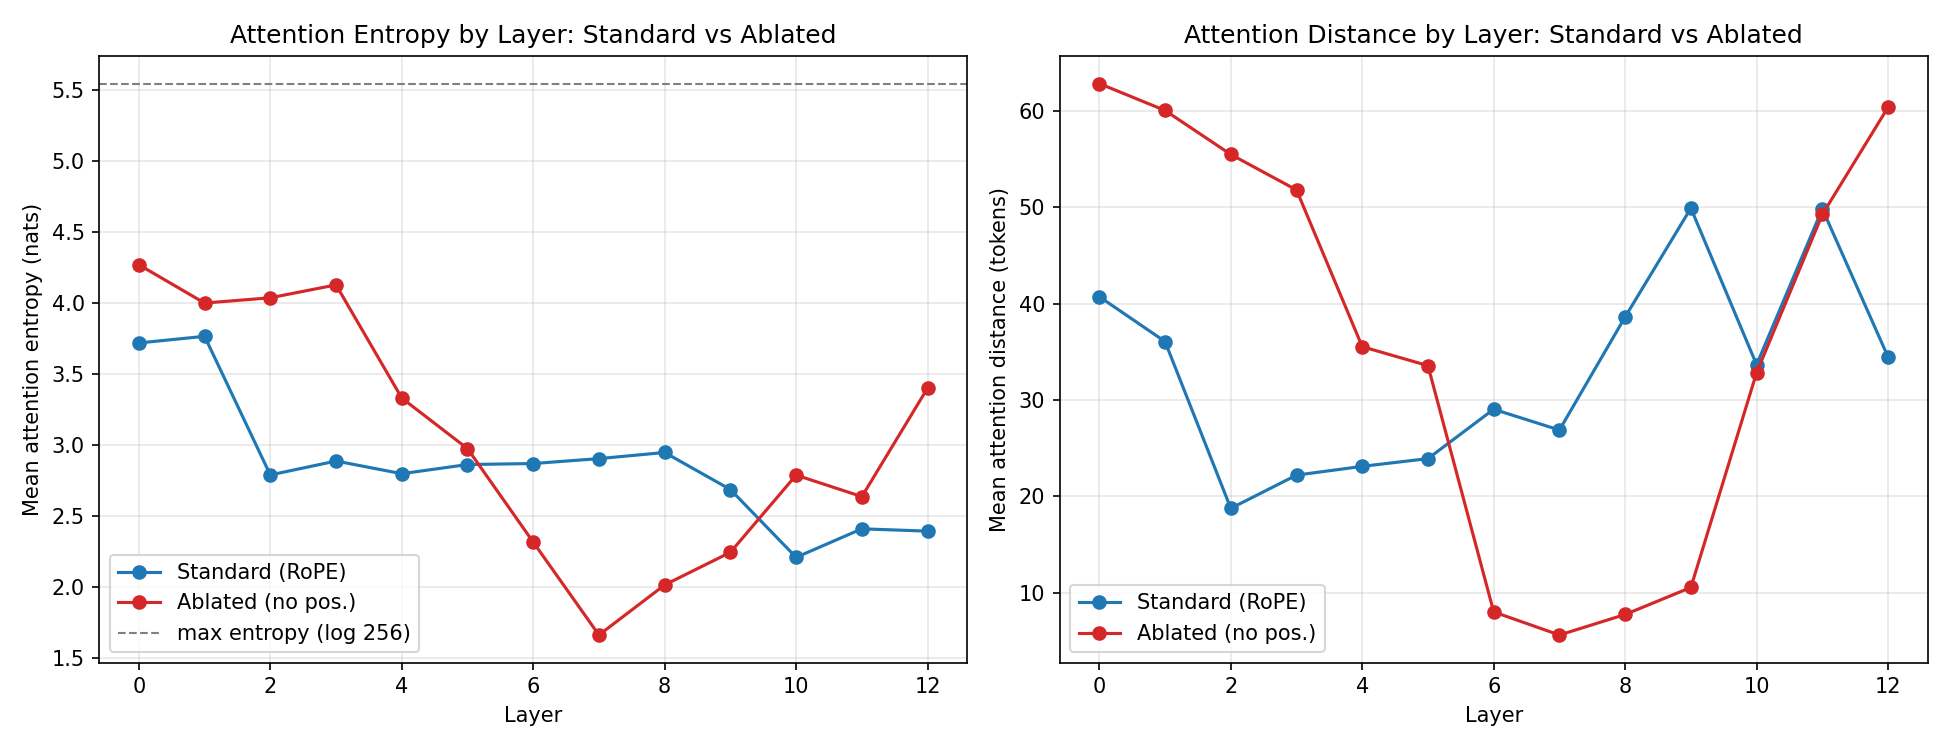
\includegraphics[width=0.48\textwidth]{../../bonus/report/plots/comparison_entropy_distance_by_layer.png}
\caption{Attention entropy and mean attention distance by layer, standard vs. ablated Hindi model. Note the crossover: the ablated model is more diffuse in early/late layers but sharper in the middle layers.}
\end{figure}

This is the most interesting result in the whole ablation, and it's the one that surprised me most. Going in, I expected the ablated model to just be spread out everywhere, since it has less information to work with. That's not what the data shows. In layers 0--3 and 10--12, attention really is much more spread out. Mean distance nearly triples at layer 2, 55.5 tokens against 18.8 for the standard model. But in layers 6--8, the ablated model's attention is actually \emph{sharper} than the standard model's, not more spread out. At layer 7, mean distance drops to 5.6 tokens compared to 26.9 for the standard model, the tightest value either model reaches at any layer.

So the network doesn't just fail evenly across all layers when position information is removed. Early and late layers, which normally get position information handed to them for free, fall back to broad, unfocused attention. But a few middle layers seem to specialize in rebuilding a rough sense of "look at my nearby tokens," using content alone. My best explanation for this: those few middle layers are spending extra effort to recover something close to what RoPE would have given the whole network for free. That effort has to come out of the same fixed number of parameters the standard model spreads more evenly across all thirteen layers, so the network partly recovers a sense of position, but only in a few layers, and at a real cost. This fits the overall pattern in this ablation: position information helps everywhere a little, but the model can only rebuild a rough, partial version of it on its own, and only in specific places.

The full writeup, with every plot and all the per-layer numbers, is on the \texttt{bonus} branch, in \path{bonus/report/ABLATION_REPORT.md}.

\section{Reproducing this project}

All the code, configs, and reports live in the GitHub repository. Google Drive links to the pretrained checkpoints, the finetuned checkpoints, and the raw corpora are in the top-level \texttt{README.md} and in each phase's own report under \texttt{report/}. The repo is organized by language (\texttt{hindi/}, \texttt{nepali/}), each with its own \texttt{tokenizer/}, \texttt{model/}, \texttt{train/}, \texttt{eval/}, \texttt{reasoning/}, and \texttt{configs/} folders, plus a shared \texttt{collection/} module for the data pipeline that gets run separately for each language. Exact commands for all three phases are in the README.

I built and tested all of this on a machine with about 7GB of RAM and not much spare swap, which shaped a few decisions beyond what's already mentioned above. The SentencePiece trainer loads its whole input sample into memory before training, so too large a sample got the process killed by the operating system twice during development (confirmed via \texttt{journalctl -k}). The fix was capping the tokenizer's training sample at 250,000 documents instead of the full corpus. Near-duplicate removal hit the same memory wall, which is why I only ran it on the crawled portion of each corpus, not on IndicCorp, as mentioned in Phase 1. There are also automated tests: \texttt{pytest tests/} for the cleaning pipeline, and separate \texttt{pytest hindi/tests/} / \texttt{pytest nepali/tests/} suites for Phase 2 covering architecture correctness, checkpoint save/resume, and the attention-analysis math, so a broken checkpoint or a wrong entropy number gets caught before I rely on it.

\end{document}
